\documentclass[a4paper]{article}
\usepackage[]{graphicx}\usepackage[]{color}
% maxwidth is the original width if it is less than linewidth
% otherwise use linewidth (to make sure the graphics do not exceed the margin)
\makeatletter
\def\maxwidth{ %
  \ifdim\Gin@nat@width>\linewidth
    \linewidth
  \else
    \Gin@nat@width
  \fi
}
\makeatother

\definecolor{fgcolor}{rgb}{0.345, 0.345, 0.345}
\newcommand{\hlnum}[1]{\textcolor[rgb]{0.686,0.059,0.569}{#1}}%
\newcommand{\hlstr}[1]{\textcolor[rgb]{0.192,0.494,0.8}{#1}}%
\newcommand{\hlcom}[1]{\textcolor[rgb]{0.678,0.584,0.686}{\textit{#1}}}%
\newcommand{\hlopt}[1]{\textcolor[rgb]{0,0,0}{#1}}%
\newcommand{\hlstd}[1]{\textcolor[rgb]{0.345,0.345,0.345}{#1}}%
\newcommand{\hlkwa}[1]{\textcolor[rgb]{0.161,0.373,0.58}{\textbf{#1}}}%
\newcommand{\hlkwb}[1]{\textcolor[rgb]{0.69,0.353,0.396}{#1}}%
\newcommand{\hlkwc}[1]{\textcolor[rgb]{0.333,0.667,0.333}{#1}}%
\newcommand{\hlkwd}[1]{\textcolor[rgb]{0.737,0.353,0.396}{\textbf{#1}}}%
\let\hlipl\hlkwb

\usepackage{framed}
\makeatletter
\newenvironment{kframe}{%
 \def\at@end@of@kframe{}%
 \ifinner\ifhmode%
  \def\at@end@of@kframe{\end{minipage}}%
  \begin{minipage}{\columnwidth}%
 \fi\fi%
 \def\FrameCommand##1{\hskip\@totalleftmargin \hskip-\fboxsep
 \colorbox{shadecolor}{##1}\hskip-\fboxsep
     % There is no \\@totalrightmargin, so:
     \hskip-\linewidth \hskip-\@totalleftmargin \hskip\columnwidth}%
 \MakeFramed {\advance\hsize-\width
   \@totalleftmargin\z@ \linewidth\hsize
   \@setminipage}}%
 {\par\unskip\endMakeFramed%
 \at@end@of@kframe}
\makeatother

\definecolor{shadecolor}{rgb}{.97, .97, .97}
\definecolor{messagecolor}{rgb}{0, 0, 0}
\definecolor{warningcolor}{rgb}{1, 0, 1}
\definecolor{errorcolor}{rgb}{1, 0, 0}
\newenvironment{knitrout}{}{} % an empty environment to be redefined in TeX

\usepackage{alltt}
\newcommand{\SweaveOpts}[1]{}  % do not interfere with LaTeX
\newcommand{\SweaveInput}[1]{} % because they are not real TeX commands
\newcommand{\Sexpr}[1]{}       % will only be parsed by R



\usepackage[utf8]{inputenc}
%\usepackage[ngerman]{babel}
\usepackage{a4wide,paralist}
\usepackage{amsmath, amssymb, xfrac, amsthm}
\usepackage{dsfont}
\usepackage[usenames,dvipsnames]{xcolor}
\usepackage{amsfonts}
\usepackage{graphicx}
\usepackage{caption}
\usepackage{subcaption}
\usepackage{framed}
\usepackage{multirow}
\usepackage{bytefield}
\usepackage{csquotes}
\usepackage[breakable, theorems, skins]{tcolorbox}
\usepackage{hyperref}
\usepackage{cancel}
\usepackage{bm}

% basic latex stuff
\newcommand{\pkg}[1]{{\fontseries{b}\selectfont #1}} % fontstyle for R packages

% Often used in exercise Rnw files, still relevant?
\newcommand{\lz}{\vspace{0.5cm}} % vertical space
\newcommand{\dlz}{\vspace{1cm}}  % double vertical space

% Unused and about to be deleted
\newcommand{\oneliner}[1] % Oneliner for important statements
{\begin{block}{}\begin{center}\begin{Large}#1\end{Large}\end{center}\end{block}}


%--------------------%
%  New environments  %
%--------------------%

 % Frame with breaks and verbatim // this is used very often
\newenvironment{vbframe}
{
\begin{frame}[containsverbatim,allowframebreaks]
}
{
\end{frame}
}

% Frame with verbatim without breaks (to avoid numbering one slided frames)
% This is not used anywhere but I can see it being useful
\newenvironment{vframe}
{
\begin{frame}[containsverbatim]
}
{
\end{frame}
}

% Itemize block
\newenvironment{blocki}[1]
{
\begin{block}{#1}\begin{itemize}
}
{
\end{itemize}\end{block}
}

%--------------%
%  Citebutton  %
%--------------%
% Example usage (from slides-cart-discussion.tex)
% \citebutton{Breiman, 1984}{https://www.taylorfrancis.com/books/mono/10.1201/9781315139470/classification-regression-trees-leo-breiman}
\newcommand{\citebutton}[2]{%
\NoCaseChange{\resizebox{!}{9pt}{\protect\beamergotobutton{\href{#2}{#1}}}}%
}

% textcolor that works in mathmode
% https://tex.stackexchange.com/a/261480
% Used e.g. in forests/slides-forests-bagging.tex
% [...] \textcolor{blue}{\tfrac{1}{M}\sum^M_{m} [...]
\makeatletter
\renewcommand*{\@textcolor}[3]{%
  \protect\leavevmode
  \begingroup
    \color#1{#2}#3%
  \endgroup
}
\makeatother


\tcbset{enhanced}

%exercise numbering
\renewcommand{\theenumi}{(\alph{enumi})}
\renewcommand{\theenumii}{\roman{enumii}}
\renewcommand\labelenumi{\theenumi}

\font \sfbold=cmssbx10
\setlength{\oddsidemargin}{0cm} \setlength{\textwidth}{16cm}

\sloppy
\parindent0em
\parskip0.5em
\topmargin-2.3 cm
\textheight25cm
\textwidth17.5cm
\oddsidemargin-0.8cm
\pagestyle{empty}

\newcommand{\kopf}[1] {
\hrule
\vspace{.15cm}
\begin{minipage}{\textwidth}
	{\sf \bf \huge Exercise collection -- #1}
\end{minipage}
\vspace{.05cm}
\hrule
\vspace{1cm}}

\newcommand{\exlect}
  {\color{black} \hrule \Large{\textbf{Lecture exercises \\}} \normalsize}
  
\newcommand{\exexams}
  {\color{black} \hrule \Large{\textbf{Questions from past exams \\}} 
  \normalsize}
  
\newcommand{\exinspo}
  {\color{black} \hrule \Large{\textbf{Ideas \& exercises from other sources 
  \\}} \normalsize}

\newcounter{aufg}
\newenvironment{aufgabe}
	{\color{black} \refstepcounter{aufg}\textbf{Exercise \arabic{aufg}:}\\ 
	\noindent}
	{\vspace{0.5cm}}
	
\newenvironment{aufgabeexam}[3] % semester, main or retry exam, question number
	{\color{black} \refstepcounter{aufg}
	\textbf{Exercise \arabic{aufg}: #1, #2 exam, question #3}\\ 
	\noindent}
	{\vspace{1.5cm}}

\newcounter{loes}
\newenvironment{loesung}
	{\color{gray} \refstepcounter{loes}\textbf{Solution \arabic{loes}:}
	\\ \noindent}
	{\bigskip}



\begin{document}
% !Rnw weave = knitr



% dependencies: amsmath, amssymb, dsfont
% math spaces
\ifdefined\N
\renewcommand{\N}{\mathds{N}} % N, naturals
\else \newcommand{\N}{\mathds{N}} \fi
\newcommand{\Z}{\mathds{Z}} % Z, integers
\newcommand{\Q}{\mathds{Q}} % Q, rationals
\newcommand{\R}{\mathds{R}} % R, reals
\ifdefined\C
\renewcommand{\C}{\mathds{C}} % C, complex
\else \newcommand{\C}{\mathds{C}} \fi
\newcommand{\continuous}{\mathcal{C}} % C, space of continuous functions
\newcommand{\M}{\mathcal{M}} % machine numbers
\newcommand{\epsm}{\epsilon_m} % maximum error

% counting / finite sets
\newcommand{\setzo}{\{0, 1\}} % set 0, 1
\newcommand{\setmp}{\{-1, +1\}} % set -1, 1
\newcommand{\unitint}{[0, 1]} % unit interval

% basic math stuff
\newcommand{\xt}{\tilde x} % x tilde
\DeclareMathOperator*{\argmax}{arg\,max} % argmax
\DeclareMathOperator*{\argmin}{arg\,min} % argmin
\newcommand{\argminlim}{\mathop{\mathrm{arg\,min}}\limits} % argmax with limits
\newcommand{\argmaxlim}{\mathop{\mathrm{arg\,max}}\limits} % argmin with limits
\newcommand{\sign}{\operatorname{sign}} % sign, signum
\newcommand{\I}{\mathbb{I}} % I, indicator
\newcommand{\order}{\mathcal{O}} % O, order
\newcommand{\bigO}{\mathcal{O}} % Big-O Landau
\newcommand{\littleo}{{o}} % Little-o Landau
\newcommand{\pd}[2]{\frac{\partial{#1}}{\partial #2}} % partial derivative
\newcommand{\floorlr}[1]{\left\lfloor #1 \right\rfloor} % floor
\newcommand{\ceillr}[1]{\left\lceil #1 \right\rceil} % ceiling
\newcommand{\indep}{\perp \!\!\! \perp} % independence symbol

% sums and products
\newcommand{\sumin}{\sum\limits_{i=1}^n} % summation from i=1 to n
\newcommand{\sumim}{\sum\limits_{i=1}^m} % summation from i=1 to m
\newcommand{\sumjn}{\sum\limits_{j=1}^n} % summation from j=1 to p
\newcommand{\sumjp}{\sum\limits_{j=1}^p} % summation from j=1 to p
\newcommand{\sumik}{\sum\limits_{i=1}^k} % summation from i=1 to k
\newcommand{\sumkg}{\sum\limits_{k=1}^g} % summation from k=1 to g
\newcommand{\sumjg}{\sum\limits_{j=1}^g} % summation from j=1 to g
\newcommand{\meanin}{\frac{1}{n} \sum\limits_{i=1}^n} % mean from i=1 to n
\newcommand{\meanim}{\frac{1}{m} \sum\limits_{i=1}^m} % mean from i=1 to n
\newcommand{\meankg}{\frac{1}{g} \sum\limits_{k=1}^g} % mean from k=1 to g
\newcommand{\prodin}{\prod\limits_{i=1}^n} % product from i=1 to n
\newcommand{\prodkg}{\prod\limits_{k=1}^g} % product from k=1 to g
\newcommand{\prodjp}{\prod\limits_{j=1}^p} % product from j=1 to p

% linear algebra
\newcommand{\one}{\bm{1}} % 1, unitvector
\newcommand{\zero}{\mathbf{0}} % 0-vector
\newcommand{\id}{\bm{I}} % I, identity
\newcommand{\diag}{\operatorname{diag}} % diag, diagonal
\newcommand{\trace}{\operatorname{tr}} % tr, trace
\newcommand{\spn}{\operatorname{span}} % span
\newcommand{\scp}[2]{\left\langle #1, #2 \right\rangle} % <.,.>, scalarproduct
\newcommand{\mat}[1]{\begin{pmatrix} #1 \end{pmatrix}} % short pmatrix command
\newcommand{\Amat}{\mathbf{A}} % matrix A
\newcommand{\Deltab}{\mathbf{\Delta}} % error term for vectors

% basic probability + stats
\renewcommand{\P}{\mathds{P}} % P, probability
\newcommand{\E}{\mathds{E}} % E, expectation
\newcommand{\var}{\mathsf{Var}} % Var, variance
\newcommand{\cov}{\mathsf{Cov}} % Cov, covariance
\newcommand{\corr}{\mathsf{Corr}} % Corr, correlation
\newcommand{\normal}{\mathcal{N}} % N of the normal distribution
\newcommand{\iid}{\overset{i.i.d}{\sim}} % dist with i.i.d superscript
\newcommand{\distas}[1]{\overset{#1}{\sim}} % ... is distributed as ...

% machine learning
\newcommand{\Xspace}{\mathcal{X}} % X, input space
\newcommand{\Yspace}{\mathcal{Y}} % Y, output space
\newcommand{\Zspace}{\mathcal{Z}} % Z, space of sampled datapoints
\newcommand{\nset}{\{1, \ldots, n\}} % set from 1 to n
\newcommand{\pset}{\{1, \ldots, p\}} % set from 1 to p
\newcommand{\gset}{\{1, \ldots, g\}} % set from 1 to g
\newcommand{\Pxy}{\mathbb{P}_{xy}} % P_xy
\newcommand{\Exy}{\mathbb{E}_{xy}} % E_xy: Expectation over random variables xy
\newcommand{\xv}{\mathbf{x}} % vector x (bold)
\newcommand{\xtil}{\tilde{\mathbf{x}}} % vector x-tilde (bold)
\newcommand{\yv}{\mathbf{y}} % vector y (bold)
\newcommand{\xy}{(\xv, y)} % observation (x, y)
\newcommand{\xvec}{\left(x_1, \ldots, x_p\right)^\top} % (x1, ..., xp)
\newcommand{\Xmat}{\mathbf{X}} % Design matrix
\newcommand{\allDatasets}{\mathds{D}} % The set of all datasets
\newcommand{\allDatasetsn}{\mathds{D}_n}  % The set of all datasets of size n
\newcommand{\D}{\mathcal{D}} % D, data
\newcommand{\Dn}{\D_n} % D_n, data of size n
\newcommand{\Dtrain}{\mathcal{D}_{\text{train}}} % D_train, training set
\newcommand{\Dtest}{\mathcal{D}_{\text{test}}} % D_test, test set
\newcommand{\xyi}[1][i]{\left(\xv^{(#1)}, y^{(#1)}\right)} % (x^i, y^i), i-th observation
\newcommand{\Dset}{\left( \xyi[1], \ldots, \xyi[n]\right)} % {(x1,y1)), ..., (xn,yn)}, data
\newcommand{\defAllDatasetsn}{(\Xspace \times \Yspace)^n} % Def. of the set of all datasets of size n
\newcommand{\defAllDatasets}{\bigcup_{n \in \N}(\Xspace \times \Yspace)^n} % Def. of the set of all datasets
\newcommand{\xdat}{\left\{ \xv^{(1)}, \ldots, \xv^{(n)}\right\}} % {x1, ..., xn}, input data
\newcommand{\ydat}{\left\{ \yv^{(1)}, \ldots, \yv^{(n)}\right\}} % {y1, ..., yn}, input data
\newcommand{\yvec}{\left(y^{(1)}, \hdots, y^{(n)}\right)^\top} % (y1, ..., yn), vector of outcomes
\newcommand{\greekxi}{\xi} % Greek letter xi
\renewcommand{\xi}[1][i]{\xv^{(#1)}} % x^i, i-th observed value of x
\newcommand{\yi}[1][i]{y^{(#1)}} % y^i, i-th observed value of y
\newcommand{\xivec}{\left(x^{(i)}_1, \ldots, x^{(i)}_p\right)^\top} % (x1^i, ..., xp^i), i-th observation vector
\newcommand{\xj}{\xv_j} % x_j, j-th feature
\newcommand{\xjvec}{\left(x^{(1)}_j, \ldots, x^{(n)}_j\right)^\top} % (x^1_j, ..., x^n_j), j-th feature vector
\newcommand{\phiv}{\mathbf{\phi}} % Basis transformation function phi
\newcommand{\phixi}{\mathbf{\phi}^{(i)}} % Basis transformation of xi: phi^i := phi(xi)

%%%%%% ml - models general
\newcommand{\lamv}{\bm{\lambda}} % lambda vector, hyperconfiguration vector
\newcommand{\Lam}{\bm{\Lambda}}	 % Lambda, space of all hpos
% Inducer / Inducing algorithm
\newcommand{\preimageInducer}{\left(\defAllDatasets\right)\times\Lam} % Set of all datasets times the hyperparameter space
\newcommand{\preimageInducerShort}{\allDatasets\times\Lam} % Set of all datasets times the hyperparameter space
% Inducer / Inducing algorithm
\newcommand{\ind}{\mathcal{I}} % Inducer, inducing algorithm, learning algorithm

% continuous prediction function f
\newcommand{\ftrue}{f_{\text{true}}}  % True underlying function (if a statistical model is assumed)
\newcommand{\ftruex}{\ftrue(\xv)} % True underlying function (if a statistical model is assumed)
\newcommand{\fx}{f(\xv)} % f(x), continuous prediction function
\newcommand{\fdomains}{f: \Xspace \rightarrow \R^g} % f with domain and co-domain
\newcommand{\Hspace}{\mathcal{H}} % hypothesis space where f is from
\newcommand{\fbayes}{f^{\ast}} % Bayes-optimal model
\newcommand{\fxbayes}{f^{\ast}(\xv)} % Bayes-optimal model
\newcommand{\fkx}[1][k]{f_{#1}(\xv)} % f_j(x), discriminant component function
\newcommand{\fh}{\hat{f}} % f hat, estimated prediction function
\newcommand{\fxh}{\fh(\xv)} % fhat(x)
\newcommand{\fxt}{f(\xv ~|~ \thetav)} % f(x | theta)
\newcommand{\fxi}{f\left(\xv^{(i)}\right)} % f(x^(i))
\newcommand{\fxih}{\hat{f}\left(\xv^{(i)}\right)} % f(x^(i))
\newcommand{\fxit}{f\left(\xv^{(i)} ~|~ \thetav\right)} % f(x^(i) | theta)
\newcommand{\fhD}{\fh_{\D}} % fhat_D, estimate of f based on D
\newcommand{\fhDtrain}{\fh_{\Dtrain}} % fhat_Dtrain, estimate of f based on D
\newcommand{\fhDnlam}{\fh_{\Dn, \lamv}} %model learned on Dn with hp lambda
\newcommand{\fhDlam}{\fh_{\D, \lamv}} %model learned on D with hp lambda
\newcommand{\fhDnlams}{\fh_{\Dn, \lamv^\ast}} %model learned on Dn with optimal hp lambda
\newcommand{\fhDlams}{\fh_{\D, \lamv^\ast}} %model learned on D with optimal hp lambda

% discrete prediction function h
\newcommand{\hx}{h(\xv)} % h(x), discrete prediction function
\newcommand{\hh}{\hat{h}} % h hat
\newcommand{\hxh}{\hat{h}(\xv)} % hhat(x)
\newcommand{\hxt}{h(\xv | \thetav)} % h(x | theta)
\newcommand{\hxi}{h\left(\xi\right)} % h(x^(i))
\newcommand{\hxit}{h\left(\xi ~|~ \thetav\right)} % h(x^(i) | theta)
\newcommand{\hbayes}{h^{\ast}} % Bayes-optimal classification model
\newcommand{\hxbayes}{h^{\ast}(\xv)} % Bayes-optimal classification model

% yhat
\newcommand{\yh}{\hat{y}} % yhat for prediction of target
\newcommand{\yih}{\hat{y}^{(i)}} % yhat^(i) for prediction of ith targiet
\newcommand{\resi}{\yi- \yih}

% theta
\newcommand{\thetah}{\hat{\theta}} % theta hat
\newcommand{\thetav}{\bm{\theta}} % theta vector
\newcommand{\thetavh}{\bm{\hat\theta}} % theta vector hat
\newcommand{\thetat}[1][t]{\thetav^{[#1]}} % theta^[t] in optimization
\newcommand{\thetatn}[1][t]{\thetav^{[#1 +1]}} % theta^[t+1] in optimization
\newcommand{\thetahDnlam}{\thetavh_{\Dn, \lamv}} %theta learned on Dn with hp lambda
\newcommand{\thetahDlam}{\thetavh_{\D, \lamv}} %theta learned on D with hp lambda
\newcommand{\mint}{\min_{\thetav \in \Theta}} % min problem theta
\newcommand{\argmint}{\argmin_{\thetav \in \Theta}} % argmin theta

% densities + probabilities
% pdf of x
\newcommand{\pdf}{p} % p
\newcommand{\pdfx}{p(\xv)} % p(x)
\newcommand{\pixt}{\pi(\xv~|~ \thetav)} % pi(x|theta), pdf of x given theta
\newcommand{\pixit}[1][i]{\pi\left(\xi[#1] ~|~ \thetav\right)} % pi(x^i|theta), pdf of x given theta
\newcommand{\pixii}[1][i]{\pi\left(\xi[#1]\right)} % pi(x^i), pdf of i-th x

% pdf of (x, y)
\newcommand{\pdfxy}{p(\xv,y)} % p(x, y)
\newcommand{\pdfxyt}{p(\xv, y ~|~ \thetav)} % p(x, y | theta)
\newcommand{\pdfxyit}{p\left(\xi, \yi ~|~ \thetav\right)} % p(x^(i), y^(i) | theta)

% pdf of x given y
\newcommand{\pdfxyk}[1][k]{p(\xv | y= #1)} % p(x | y = k)
\newcommand{\lpdfxyk}[1][k]{\log p(\xv | y= #1)} % log p(x | y = k)
\newcommand{\pdfxiyk}[1][k]{p\left(\xi | y= #1 \right)} % p(x^i | y = k)

% prior probabilities
\newcommand{\pik}[1][k]{\pi_{#1}} % pi_k, prior
\newcommand{\lpik}[1][k]{\log \pi_{#1}} % log pi_k, log of the prior
\newcommand{\pit}{\pi(\thetav)} % Prior probability of parameter theta

% posterior probabilities
\newcommand{\post}{\P(y = 1 ~|~ \xv)} % P(y = 1 | x), post. prob for y=1
\newcommand{\postk}[1][k]{\P(y = #1 ~|~ \xv)} % P(y = k | y), post. prob for y=k
\newcommand{\pidomains}{\pi: \Xspace \rightarrow \unitint} % pi with domain and co-domain
\newcommand{\pibayes}{\pi^{\ast}} % Bayes-optimal classification model
\newcommand{\pixbayes}{\pi^{\ast}(\xv)} % Bayes-optimal classification model
\newcommand{\pix}{\pi(\xv)} % pi(x), P(y = 1 | x)
\newcommand{\piv}{\bm{\pi}} % pi, bold, as vector
\newcommand{\pikx}[1][k]{\pi_{#1}(\xv)} % pi_k(x), P(y = k | x)
\newcommand{\pikxt}[1][k]{\pi_{#1}(\xv ~|~ \thetav)} % pi_k(x | theta), P(y = k | x, theta)
\newcommand{\pixh}{\hat \pi(\xv)} % pi(x) hat, P(y = 1 | x) hat
\newcommand{\pikxh}[1][k]{\hat \pi_{#1}(\xv)} % pi_k(x) hat, P(y = k | x) hat
\newcommand{\pixih}{\hat \pi(\xi)} % pi(x^(i)) with hat
\newcommand{\pikxih}[1][k]{\hat \pi_{#1}(\xi)} % pi_k(x^(i)) with hat
\newcommand{\pdfygxt}{p(y ~|~\xv, \thetav)} % p(y | x, theta)
\newcommand{\pdfyigxit}{p\left(\yi ~|~\xi, \thetav\right)} % p(y^i |x^i, theta)
\newcommand{\lpdfygxt}{\log \pdfygxt } % log p(y | x, theta)
\newcommand{\lpdfyigxit}{\log \pdfyigxit} % log p(y^i |x^i, theta)

% probababilistic
\newcommand{\bayesrulek}[1][k]{\frac{\P(\xv | y= #1) \P(y= #1)}{\P(\xv)}} % Bayes rule
\newcommand{\muk}{\bm{\mu_k}} % mean vector of class-k Gaussian (discr analysis)

% residual and margin
\newcommand{\eps}{\epsilon} % residual, stochastic
\newcommand{\epsv}{\bm{\epsilon}} % residual, stochastic, as vector
\newcommand{\epsi}{\epsilon^{(i)}} % epsilon^i, residual, stochastic
\newcommand{\epsh}{\hat{\epsilon}} % residual, estimated
\newcommand{\epsvh}{\hat{\epsv}} % residual, estimated, vector
\newcommand{\yf}{y \fx} % y f(x), margin
\newcommand{\yfi}{\yi \fxi} % y^i f(x^i), margin
\newcommand{\Sigmah}{\hat \Sigma} % estimated covariance matrix
\newcommand{\Sigmahj}{\hat \Sigma_j} % estimated covariance matrix for the j-th class

% ml - loss, risk, likelihood
\newcommand{\Lyf}{L\left(y, f\right)} % L(y, f), loss function
\newcommand{\Lypi}{L\left(y, \pi\right)} % L(y, pi), loss function
\newcommand{\Lxy}{L\left(y, \fx\right)} % L(y, f(x)), loss function
\newcommand{\Lxyi}{L\left(\yi, \fxi\right)} % loss of observation
\newcommand{\Lxyt}{L\left(y, \fxt\right)} % loss with f parameterized
\newcommand{\Lxyit}{L\left(\yi, \fxit\right)} % loss of observation with f parameterized
\newcommand{\Lxym}{L\left(\yi, f\left(\bm{\tilde{x}}^{(i)} ~|~ \thetav\right)\right)} % loss of observation with f parameterized
\newcommand{\Lpixy}{L\left(y, \pix\right)} % loss in classification
\newcommand{\Lpiv}{L\left(y, \piv\right)} % loss in classification
\newcommand{\Lpixyi}{L\left(\yi, \pixii\right)} % loss of observation in classification
\newcommand{\Lpixyt}{L\left(y, \pixt\right)} % loss with pi parameterized
\newcommand{\Lpixyit}{L\left(\yi, \pixit\right)} % loss of observation with pi parameterized
\newcommand{\Lhxy}{L\left(y, \hx\right)} % L(y, h(x)), loss function on discrete classes
\newcommand{\Lr}{L\left(r\right)} % L(r), loss defined on residual (reg) / margin (classif)
\newcommand{\lone}{|y - \fx|} % L1 loss
\newcommand{\ltwo}{\left(y - \fx\right)^2} % L2 loss
\newcommand{\lbernoullimp}{\ln(1 + \exp(-y \cdot \fx))} % Bernoulli loss for -1, +1 encoding
\newcommand{\lbernoullizo}{- y \cdot \fx + \log(1 + \exp(\fx))} % Bernoulli loss for 0, 1 encoding
\newcommand{\lcrossent}{- y \log \left(\pix\right) - (1 - y) \log \left(1 - \pix\right)} % cross-entropy loss
\newcommand{\lbrier}{\left(\pix - y \right)^2} % Brier score
\newcommand{\risk}{\mathcal{R}} % R, risk
\newcommand{\riskbayes}{\mathcal{R}^\ast}
\newcommand{\riskf}{\risk(f)} % R(f), risk
\newcommand{\riskdef}{\E_{y|\xv}\left(\Lxy \right)} % risk def (expected loss)
\newcommand{\riskt}{\mathcal{R}(\thetav)} % R(theta), risk
\newcommand{\riske}{\mathcal{R}_{\text{emp}}} % R_emp, empirical risk w/o factor 1 / n
\newcommand{\riskeb}{\bar{\mathcal{R}}_{\text{emp}}} % R_emp, empirical risk w/ factor 1 / n
\newcommand{\riskef}{\riske(f)} % R_emp(f)
\newcommand{\risket}{\mathcal{R}_{\text{emp}}(\thetav)} % R_emp(theta)
\newcommand{\riskr}{\mathcal{R}_{\text{reg}}} % R_reg, regularized risk
\newcommand{\riskrt}{\mathcal{R}_{\text{reg}}(\thetav)} % R_reg(theta)
\newcommand{\riskrf}{\riskr(f)} % R_reg(f)
\newcommand{\riskrth}{\hat{\mathcal{R}}_{\text{reg}}(\thetav)} % hat R_reg(theta)
\newcommand{\risketh}{\hat{\mathcal{R}}_{\text{emp}}(\thetav)} % hat R_emp(theta)
\newcommand{\LL}{\mathcal{L}} % L, likelihood
\newcommand{\LLt}{\mathcal{L}(\thetav)} % L(theta), likelihood
\newcommand{\LLtx}{\mathcal{L}(\thetav | \xv)} % L(theta|x), likelihood
\newcommand{\logl}{\ell} % l, log-likelihood
\newcommand{\loglt}{\logl(\thetav)} % l(theta), log-likelihood
\newcommand{\logltx}{\logl(\thetav | \xv)} % l(theta|x), log-likelihood
\newcommand{\errtrain}{\text{err}_{\text{train}}} % training error
\newcommand{\errtest}{\text{err}_{\text{test}}} % test error
\newcommand{\errexp}{\overline{\text{err}_{\text{test}}}} % avg training error

% lm
\newcommand{\thx}{\thetav^\top \xv} % linear model
\newcommand{\olsest}{(\Xmat^\top \Xmat)^{-1} \Xmat^\top \yv} % OLS estimator in LM


\kopf{Supervised Classification}

% ------------------------------------------------------------------------------
% LECTURE EXERCISES
% ------------------------------------------------------------------------------

\exlect
\lz

\aufgabe{

In logistic regression, we estimate the probability $\pix = \post$.
To decide if $\hat{y}$ is $0$ or $1$, we follow:

$$
\hat{y} = 1 \ \ \Leftrightarrow \ \ \pixh \geq a
$$


\begin{itemize}
\item[a)] What happens if you are choosing $a = 0.5$? More precisely, from which value of $\thetab^T \xv$ do you predict $\hat{y} = 1$ rather than $\hat{y} = 0$?
\item[b)] Explain (using words) why $a = 0.5$ is a sensible threshold.
\end{itemize}
}

\dlz
\loesung{

\begin{enumerate}
\item %Logistic regression is a classification model, that estimates posterior probabilities $\pi(x)$ by linear functions in $x$.
For a binary classification problem the model can be written as:\\

$$
\hat{y} = 1 \ \ \Leftrightarrow \ \ \pix = \frac{1}{1 + \exp(-\thetab^T \xv)} \geq a
$$

This can be reformulated, s.t. for $a \in (0,1)$

\begin{align*}
&\frac{1}{1 + \exp(-\thetab^T \xv)} \geq a \\
\Leftrightarrow\ & 1 + \exp(-\thetab^T \xv) \leq a^{-1} \\
\Leftrightarrow\ & \exp(-\thetab^T \xv) \leq a^{-1} - 1 \\
\Leftrightarrow\ & -\thetab^T \xv \leq \log(a^{-1} - 1) \\
\Leftrightarrow\ & \thetab^T \xv \geq -\log(a^{-1} - 1) \\
\end{align*}



For $a = 0.5$ we get:

$$
\hat{y} = 1 \ \ \Leftrightarrow \ \ \thetab^T \xv \geq -\log(0.5^{-1} - 1) = -\log(2 - 1) = -\log(1) = 0
$$
This means the linear decision boundary is defined by a hyperplane equation, i.e.,  
$\thetab^T \xv = 0$
and it divides the input space in the "1"-space ($\thetab^T \xv \geq 0$) and in the "0"-space ($\thetab^T \xv < 0$).
\item  When the threshold $a = 0.5$ is chosen, the losses of missclassified observations, i.e., $L(\hat{y}=0|y=1)$ and  $L(\hat{y}=1|y=0)$ ,  are weighted equally. This means $a = 0.5$ is a sensible threshold if one does not need to avoid one type of misclassification more than the other.\\
Intuitively it makes sense to cut off at $0.5$ because, if the probability for 1 is closer to 1 than to 0, we would intuitively choose 1 rather than 0.
\end{enumerate}
}

\aufgabe{

\begin{enumerate}
  \item[a)] What is the relationship between softmax $\pi_k(x)=\frac{\exp(\theta_k^T x)}{\sum^g_{j=1} \exp(\theta_j^T x)}$ and the logistic function $\pix =\frac{1}{1+\exp(-\theta^{T} x)}$ for $g = 2$ (binary classification)?

  \item[b)] The likelihood function of a multinomially distributed target variable with $g$ target classes is given by
 $$\mathcal{L}_i = \P(Y^{(i)} = y^{(i)}|x^{(i)},\theta_1, \dots, \theta_g) = 
\prod^g_{j=1} \pi_j(x^{(i)})^{\mathds{1}_{\{y^{(i)} = j\}}}$$
where the posterior class probablities $\pi_1(x), \dots, \pi_g(x)$ are modeled with softmax regression.
  Derive the likelihood function of $n$ such independent target variables. How can you transform this likelihood function into an empirical risk function?
  \\ Hints: 
  \begin{itemize}
  \item By following the maximum likelihood principle, we should look for parameters $\theta_1, \dots, \theta_g$, which maximize the likelihood function.
  \item The expressions $\prod \mathcal{L}_i$ and $\log\prod\mathcal{L}_i$ (if this expression is defined) are maximized by the same parameters.
  \item The empirical risk is a \emph{sum} of loss function values, not a \emph{product}.
  \item Minimizing a scalar function multiplied with -1 is equivalent to maximizing the original function.
  \end{itemize}
  State the associated loss function. 

  \item[c)] Explain how the predictions of softmax regression (multiclass classification) look like (probabilities and classes) and define the parameter space.

  % \item[c)] Calculate the derivative of the negative likelihood as a loss function for softmax regression: $\triangledown_{\theta_k}L= \sum_{i=1}^n {-x ([y[i]==k] - \pi_k)}$ (suppose there are n instances)
\end{enumerate}

}
\dlz
\loesung{

\begin{enumerate}

  \item[a)]

  $\pi_1(x)=\frac{\exp(\theta_1^T x)}{\exp(\theta_1^T x) + \exp(\theta_2^T x)}$

  $\pi_2(x)=\frac{\exp(\theta_2^T x)}{\exp(\theta_1^T x) + \exp(\theta_2^T x)}$

  $\pi_1(x)=\frac{1}{ (\exp(\theta_1^T x) + \exp(\theta_2^T x) )/ \exp(\theta_1^T x)} = \frac{1}{1+\exp(-\theta^{T} x)}$ where $\theta =\theta_1 - \theta_2 $ and $\pi_2(x) = 1 - \pi_1(x)$

  \item[b)]
  When using softmax regression the posterior class probability for the class $k$ is modeled, s.t.
  $$\pi_k(x) = \frac{\exp(\theta_k^T x)}{\sum^g_{j=1} \exp(\theta_j^T x)}.$$ 
  
  A single observation is multinomially distributed, i.e., 
$$\mathcal{L}_i = \P(Y^{(i)} = y^{(i)}|x^{(i)},\theta_1, \dots, \theta_g) = 
\prod^g_{j=1} \pi_j(x^{(i)})^{\mathds{1}_{\{y^{(i)} = j\}}}.$$
  Under the assumption that the observations are conditionally independent the 
  likelihood of the data can be expressed, s.t.
  $$\mathcal{L} = \P(Y^{(1)} = y^{(1)},\dots,Y^{(n)} = y^{(n)}|x^{(1)},\dots,x^{(n)},\theta_1, \dots, \theta_g) = \prod^n_{i=1}\prod^g_{j=1} \pi_j(x^{(i)})^{\mathds{1}_{\{y^{(i)} = j\}}}.$$
(By following the maximum likelihood principle, we should look for parameters $\theta_1, \dots, \theta_g$, which maximize the expression above.) \\
 Now we want the empirical risk to be a \emph{sum} of loss function values, not a \emph{product}
recall: $$\riske = \sum^n_{i=1} \Lxyi.$$
We can turn the product into a sum by taking its log since the same parameters maximize the expressions. Finally, we convert the maximization into minimization by multiplying with -1. So we end up with the so-called cross-entropy loss function:
  
$$ \Lxy = -\sum^g_{j=1} \mathds{1}_{\{y = j\}}\log[{\pi_j(x)}].$$
 
We see that for the softmax regression the loss function is equal to the negative log-likelihood of one observation. Thus the associated empirical risk is the negative log-likelihood of the complete data set.
  
  \item[c)]
  Since the subtraction of any fixed vector from all $\theta_k$ does not change the prediction, one set of parameters is "redundant". Thus we set $\theta_g = (0,\dots,0).$
    Hence for $g$ classes we get $g - 1$ discriminant functions from the softmax $\hat{\pi}_1(x), \dots, \hat{\pi}_{g-1}(x)$ which can be interpreted as probability. The probability for class $g$ can be calculated by using $\hat{\pi}_g = 1 - \sum_{k = 1}^{g-1} \hat{\pi}_k(x)$. To estimate the class we are using majority vote:
    $$
    \hat{y} = \argmax_k \hat{\pi}_k(x)
    $$
    The parameter of the softmax regression is defined as parameter matrix where each class has its own parameter vector $\theta_k$, $k \in \{1, \dots, g-1\}$:
    $$
    \theta = [\theta_1, \dots, \theta_{g-1}]
    $$



  % $\frac{\partial (-\log L)}{\partial \theta_i} = - \sum_k I_k \frac{1}{\pi_k} \frac{\partial \pi_k}{\partial \theta_i}$

  % since

  % $ \frac{\partial \pi_i}{\partial \theta_i} = \triangledown_{\theta_i} \frac{e^{\theta_i^T x}}{\sum_k e^{\theta_k^T x}}= \frac{e^{z_i}(\sum_k e^{z_k})-(e^{z_i})^2}{(\sum_k e^{z_k})^2}x = \frac{e^{z_i}(\sum_{k \neq i} e^{z_k})}{(\sum_k e^{z_k})^2}x= \pi_i(1 - \pi_i)x$,

  % $ \frac{\partial \pi_i}{\partial \theta_j} = \triangledown_{\theta_j} \frac{e^{\theta_i^T x}}{\sum_k e^{\theta_k^T x}}= \frac{-e^{z_i}e^{z_j}}{(\sum_k e^{z_k})^2}x= - \pi_i\pi_j x$, ($i \neq j$)

  % Conclusion:

  % $\frac{- \partial \log L}{\partial \theta_i} = - \sum_k I_k \frac{1}{\pi_k} \frac{\partial \pi_k}{\partial \theta_i} = -(1-\pi_i)x$ ($i = y$)
  % and

  % $\frac{- \partial \log L}{\partial \theta_j} = - \sum_k I_k \frac{1}{\pi_k} \frac{\partial \pi_k}{\partial \theta_j} = \pi_j x$
  % ($j \neq y$)

  % Writing the two cases in one formula, we have

  % $\frac{- \partial \log L}{\partial \theta_k} = -(I_k -\pi_k )x$ where $I_k = [y = k]$

  % summing over all instances, we have

  % $\triangledown_{\theta_k}\mathcal{L} = \sum_{i=1}^n-([y_i = k] -\pi_k )x$
\end{enumerate}

}

\aufgabe{

Choose some of the classifiers already introduced in the lecture and visualize their decision boundaries for relevant hyperparameters.
Use \texttt{mlbench::mlbench.spirals} to generate data and use \texttt{plot\_learner\_prediction} for visualization. To refresh your knowledge about \texttt{mlr3} you can take a look at \url{https://mlr3book.mlr-org.com/basics.html}.

}
\dlz
\loesung{

See \href{https://github.com/compstat-lmu/lecture_i2ml/blob/master/exercises/supervised-classification/sol_mlr_dec_boundaries.R}{R code}
}
\dlz

\aufgabe{

%x <- c(4,7,9,4,6,7,9,7,8)
%y <- c(6,3,8,9,5,8,7,6,5)
%z <- as.factor(c(1,1,1,0,0,0,0,2,1))

Let the 2D feature vectors in the following figure be with two different class labels (triangles
and circles). Classify the point (7,6) - represented by a square in the picture - with
a k-nearest neighbor classifier. Distance function should be the $L_1$ norm (Manhattan distance):

$$d_\text{manhattan}(x, \tilde{x}) = \sum_{j=1}^p |x_j - \tilde{x}_j|$$

As a decision rule, use the unweighted number of the individual classes in the k-next
Neighbor Quantity, i.\,e.\ the point is assigned to the class that represents most k-nearest neighbors.

\begin{itemize}
  \item[a)] $k = 3$
  \item[b)] $k = 5$
  \item[c)] $k = 7$
\end{itemize}

%d3 = c(5,7,9,7)
%v3 = c(6,8,6,4)

%d5 = c(4,7,10,7)
%v5 = c(6,9,6,3)

%d7 = c(3,7,10,10,7)
%v7 = c(6,10,7,5,2)



\begin{knitrout}
\definecolor{shadecolor}{rgb}{0.969, 0.969, 0.969}\color{fgcolor}

{\centering 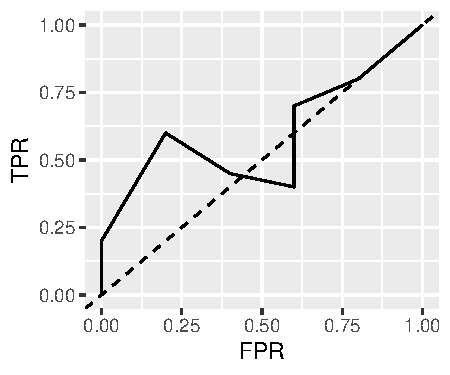
\includegraphics[width=\maxwidth]{figure/unnamed-chunk-16-1} 

}


\end{knitrout}
}
\dlz
\loesung{

\begin{enumerate}
\item[a)] $k = 3$

2 circles and 1 triangle, so our point is also a circle

\begin{knitrout}
\definecolor{shadecolor}{rgb}{0.969, 0.969, 0.969}\color{fgcolor}

{\centering 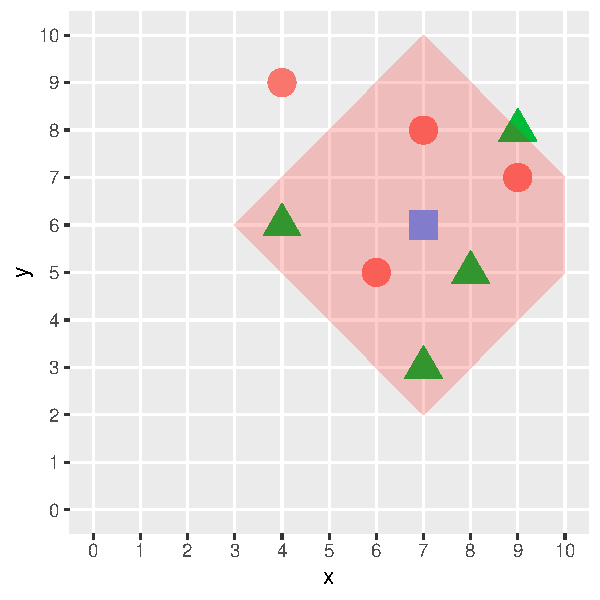
\includegraphics[width=\maxwidth]{figure/unnamed-chunk-17-1} 

}


\end{knitrout}

\item[b)] $k = 5$

3 circles and 3 triangles, we have to specify beforehand what to do in case of a tie

\begin{knitrout}
\definecolor{shadecolor}{rgb}{0.969, 0.969, 0.969}\color{fgcolor}

{\centering 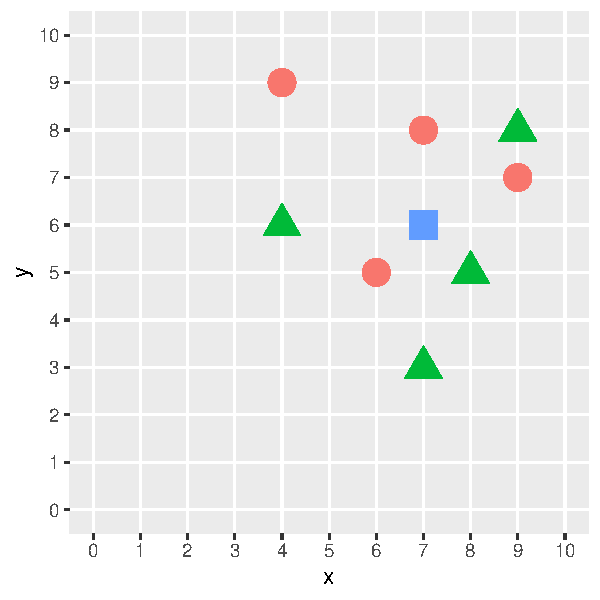
\includegraphics[width=\maxwidth]{figure/unnamed-chunk-18-1} 

}


\end{knitrout}

\item[c)] $k = 7$

3 circles and 4 triangles, so our point is also a triangle

\begin{knitrout}
\definecolor{shadecolor}{rgb}{0.969, 0.969, 0.969}\color{fgcolor}

{\centering 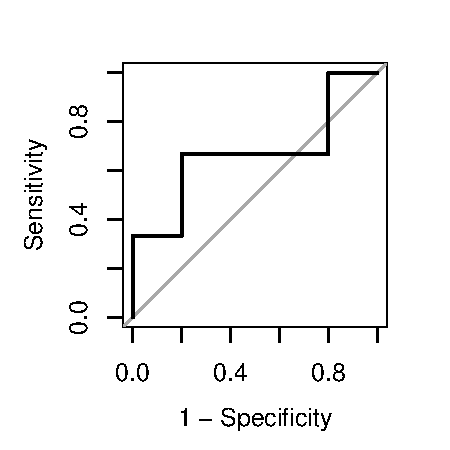
\includegraphics[width=\maxwidth]{figure/unnamed-chunk-19-1} 

}


\end{knitrout}

\end{enumerate}


  
}
\newpage

\aufgabe{

You are given the following table with the target variable \texttt{Banana}:
\begin{center}
\begin{tabular}{ | c | c | c | c | c |}
\hline
ID  &  Color   &  Form    &  Origin    &  Banana ?  \\  \hline
1   &  yellow  &  oblong  &  imported  &  yes       \\
2   &  yellow  &  round   &  domestic  &  no        \\
3   &  yellow  &  oblong  &  imported  &  no        \\
4   &  brown   &  oblong  &  imported  &  yes       \\
5   &  brown   &  round   &  domestic  &  no        \\
6   &  green   &  round   &  imported  &  yes       \\
7   &  green   &  oblong  &  domestic  &  no        \\
8   &  red     &  round   &  imported  &  no        \\
\hline
\end{tabular}
\end{center}

\begin{enumerate}
  \item[a)]
    We want to use a naive Bayes classifier to predict whether a new fruit is a Banana or not. Calculate the posterior probability $\pi(x)$ for a new observation $(\text{yellow}, \text{round}, \text{imported})$. How would you classify the object?

  \item[b)]
    Assume you have an additional feature "Length", which measures the length in cm. Describe in 1-2 sentences how you would handle this numeric feature with Naive Bayes.
\end{enumerate}
}
\dlz
\loesung{

\begin{enumerate}

  \item[a)]

When using the naive Bayes classifier, the features $x := (x_\text{Color},x_\text{Form},x_\text{Origin})$ given the category $y \in \{\text{yes},\text{no}\}$ are assumed to be conditionally independent of each other, s.t.

$$p((x_\text{Color},x_\text{Form},x_\text{Origin})|y = k) = p(x_\text{Color}|y = k)\cdot p(x_\text{Form}|y = k) \cdot p(x_\text{Origin}|y = k).$$

For the posterior probabilities $\pi_k(x)$ it holds that
\begin{align*} \pi_k(x) \propto & \; \underbrace{\pi_k \cdot p(x_\text{Color}|y = k)\cdot p(x_\text{Form}|y = k) \cdot p(x_\text{Origin}|y = k)}_{=: \alpha_k(x)} \\
\iff & \exists c \in \mathbb{R}: \pi_k(x) = c \cdot \alpha_k(x),\end{align*}
where $\pi_k$ is the prior probability of class $k$.
From this and since the posterior probabilities need to sum up to 1, it holds that 
\begin{align*}1 =& \; c \cdot \alpha_\text{yes}(x) +  c \cdot \alpha_\text{no}(x)\\
\iff & c = \frac{1}{\alpha_\text{yes}(x) + \alpha_\text{no}(x)}.
\end{align*}
This means in order to compute $\pi_\text{yes}(x)$ the scores $\alpha_\text{yes}(x)$ and $\alpha_\text{no}(x)$ are needed.\\ Now we want to compute for a new fruit the posterior probability $\hat{\pi}_{yes}((\text{yellow},\text{round},\text{imported}))$. \\
Note that we do not know the \emph{true} prior probability and the \emph{true} conditional densities. Here -since the target and the features are categorical- we can estimate them with the relative frequencies encountered in the data, s.t.
\begin{align*}
\hat{\alpha}_\text{yes}(x) = & \;  \hat{\pi}_{yes} \cdot \hat{p}(\text{yellow}|y = \text{yes})\cdot \hat{p}(\text{round}|y = \text{yes}) \cdot \hat{p}(\text{imported}|y = \text{yes}) \\
= & \; \hat{\P}(y = \text{yes}) \cdot \hat{\P}(x_\text{Color} = \text{yellow}|y = \text{yes})\cdot \hat{\P}(x_\text{Form}=\text{round}|y = \text{yes}) \cdot \hat{\P}(x_\text{Origin}=\text{imported}|y = \text{yes}) \\
= & \; \frac{3}{8} \cdot \frac{1}{3} \cdot \frac{1}{3} \cdot 1 = \frac{1}{24} \approx 0.042, \\
\hat{\alpha}_\text{no}(x) = & \;  \hat{\pi}_{no} \cdot \hat{p}(\text{yellow}|y = \text{no})\cdot \hat{p}(\text{round}|y = \text{no}) \cdot \hat{p}(\text{imported}|y = \text{no}) \\
= & \; \hat{\P}(y = \text{no}) \cdot \hat{\P}(x_\text{Color} = \text{yellow}|y = \text{no})\cdot \hat{\P}(x_\text{Form}=\text{round}|y = \text{no}) \cdot \hat{\P}(x_\text{Origin}=\text{imported}|y = \text{no}) \\
= & \; \frac{5}{8} \cdot \frac{2}{5} \cdot \frac{3}{5} \cdot \frac{2}{5} = \frac{3}{50} = 0.06.
\end{align*}
At this stage we can already see that the predicted label is "no", since $ \hat{\alpha}_\text{no}(x) = 0.06>\frac{1}{24} = 
\hat{\alpha}_\text{yes}(x)$. \\
With this we can calculate the posterior probability
$$\hat{\pi}_\text{yes}(x) = \frac{\hat{\alpha}_\text{yes}(x)}{\hat{\alpha}_\text{yes}(x) + \hat{\alpha}_\text{no}(x)} \approx 0.41.$$


    Corresponding \texttt{R}-Code:

\begin{knitrout}
\definecolor{shadecolor}{rgb}{0.969, 0.969, 0.969}\color{fgcolor}\begin{kframe}
\begin{alltt}
\hlstd{df_banana} \hlkwb{<-} \hlkwd{data.frame}\hlstd{(}
  \hlkwc{Color} \hlstd{=} \hlkwd{as.factor}\hlstd{(}
    \hlkwd{c}\hlstd{(}\hlstr{"yellow"}\hlstd{,} \hlstr{"yellow"}\hlstd{,} \hlstr{"yellow"}\hlstd{,} \hlstr{"brown"}\hlstd{,} \hlstr{"brown"}\hlstd{,} \hlstr{"green"}\hlstd{,} \hlstr{"green"}\hlstd{,} \hlstr{"red"}\hlstd{)),}
  \hlkwc{Form} \hlstd{=} \hlkwd{as.factor}\hlstd{(}
    \hlkwd{c}\hlstd{(}\hlstr{"oblong"}\hlstd{,} \hlstr{"round"}\hlstd{,} \hlstr{"oblong"}\hlstd{,} \hlstr{"oblong"}\hlstd{,} \hlstr{"round"}\hlstd{,} \hlstr{"round"}\hlstd{,} \hlstr{"oblong"}\hlstd{,} \hlstr{"round"}\hlstd{)),}
  \hlkwc{Origin} \hlstd{=} \hlkwd{as.factor}\hlstd{(}
    \hlkwd{c}\hlstd{(}\hlstr{"imported"}\hlstd{,} \hlstr{"domestic"}\hlstd{,} \hlstr{"imported"}\hlstd{,} \hlstr{"imported"}\hlstd{,} \hlstr{"domestic"}\hlstd{,} \hlstr{"imported"}\hlstd{,}
    \hlstr{"domestic"}\hlstd{,} \hlstr{"imported"}\hlstd{)),}
  \hlkwc{Banana} \hlstd{=} \hlkwd{as.factor}\hlstd{(}\hlkwd{c}\hlstd{(}\hlstr{"yes"}\hlstd{,} \hlstr{"no"}\hlstd{,} \hlstr{"no"}\hlstd{,} \hlstr{"yes"}\hlstd{,} \hlstr{"no"}\hlstd{,} \hlstr{"yes"}\hlstd{,} \hlstr{"no"}\hlstd{,} \hlstr{"no"}\hlstd{))}
\hlstd{)}

\hlstd{new_fruit} \hlkwb{<-} \hlkwd{data.frame}\hlstd{(}\hlkwc{Color} \hlstd{=} \hlstr{"yellow"}\hlstd{,} \hlkwc{Form} \hlstd{=} \hlstr{"round"}\hlstd{,} \hlkwc{Origin} \hlstd{=} \hlstr{"imported"}\hlstd{,} \hlkwc{Banana} \hlstd{=} \hlnum{NA}\hlstd{)}
\hlstd{df_banana} \hlkwb{<-} \hlkwd{rbind}\hlstd{(df_banana, new_fruit)}

\hlkwd{library}\hlstd{(mlr3)}
\hlkwd{library}\hlstd{(mlr3learners)}

\hlstd{nb_learner} \hlkwb{<-} \hlkwd{lrn}\hlstd{(}\hlstr{"classif.naive_bayes"}\hlstd{,}
                  \hlkwc{predict_type} \hlstd{=} \hlstr{"prob"}\hlstd{)}

\hlstd{banana_task} \hlkwb{<-} \hlstd{TaskClassif}\hlopt{$}\hlkwd{new}\hlstd{(}
  \hlkwc{id} \hlstd{=} \hlstr{"banana"}\hlstd{,}
  \hlkwc{backend} \hlstd{= df_banana,}
  \hlkwc{target} \hlstd{=} \hlstr{"Banana"}
\hlstd{)}

\hlstd{nb_learner}\hlopt{$}\hlkwd{train}\hlstd{(banana_task,} \hlkwc{row_ids}\hlstd{=}\hlnum{1}\hlopt{:}\hlnum{8}\hlstd{)}

\hlstd{nb_learner}\hlopt{$}\hlkwd{predict}\hlstd{(banana_task,} \hlkwc{row_ids} \hlstd{=} \hlnum{9}\hlstd{)}
\end{alltt}
\begin{verbatim}
## <PredictionClassif> for 1 observations:
##  row_ids truth response   prob.no  prob.yes
##        9  <NA>       no 0.5901639 0.4098361
\end{verbatim}
\end{kframe}
\end{knitrout}

  \item[b)]
    For the distribution of a numerical feature given the the category we need to specify a probability distribution with continuous support.
    For example, for the information $x_\text{Length}$ we could assume that $p(x_\text{Length} | y = \text{yes}) \sim \mathcal{N}(\mu_\text{yes},\sigma^2_\text{yes})$ and $p(x_\text{Length} | y = \text{no}) \sim \mathcal{N}(\mu_\text{no},\sigma^2_\text{no})$. (To estimate these normal distributions one would need to estimate their parameters $\mu_\text{yes},\mu_\text{no},\sigma^2_\text{yes},\sigma^2_\text{no}$ on the data respectively)
\end{enumerate}
}

\newpage

% ------------------------------------------------------------------------------
% PAST EXAMS
% ------------------------------------------------------------------------------

\dlz
\exexams
\lz

\aufgabeexam{WS2020/21}{main}{1}{

\begin{knitrout}
\definecolor{shadecolor}{rgb}{0.969, 0.969, 0.969}\color{fgcolor}

{\centering 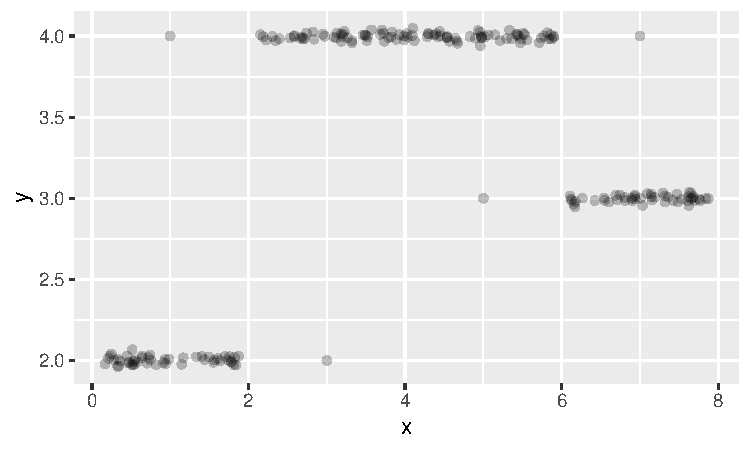
\includegraphics[width=\maxwidth]{figure/unnamed-chunk-10-1} 

}


\end{knitrout}

The above plot shows $\D = \Dset $, a data set with %$n$ observations
%data $\xv = (x^{(1)}, \dots, x^{(n)})^\top$ and $\ydat = \yvec$ for 
$n$ = 200 observations of a continuous target variable $y$ and a continuous, 
1-dimensional feature variable $\xv$. In the following, we aim at predicting 
$y$ with a machine learning model that takes $\xv$ as input.

\begin{enumerate}
  \item Since the data seem to fall in 3 quite well-separable classes, we now 
  want to apply a classification model instead of the regression model in a). 
  To prepare the data for classification, we categorize the target variable $y$ 
  in 3 classes and call the transformed target variable $z$, as follows:
  \[
    z^{(i)} = \left\{\begin{array}{lr}
        1, \text{ if }&  -\infty < \yi \leq 2.5 \\
        2, \text{ if }&  2.5\ < \yi \leq 3.5 \\
        3, \text{ if }&  3.5 < \yi < \infty
        \end{array} \right\}
  \]
  Now we can apply quadratic discriminant analysis (QDA):
  \begin{enumerate}
    \item[(i)] Estimate the class means $\mu_k = \E(\xv|z = k)$ for each of the 
    three classes $k \in \{1, 2, 3\}$ visually from the plot. Do not 
    overcomplicate this, a rough estimate is sufficient here.
    \item[(ii)] Make a hand-drawn plot that visualizes the different estimated 
    densities per class.
    \item[(iii)] How would your drawing from (ii) change if we used linear 
    discriminant analysis (LDA) instead of QDA? Explain your answer.
    \item[(iv)] Why is QDA for this data preferable over LDA?
  \end{enumerate}  
  \item Given are two new observations $\xv_{*1} = -10$ and $\xv_{*2} = 7$. 
  State the prediction for each of the two models 
  \begin{enumerate}
    \item[(i)] regression tree (from a))
    \item[(ii)] QDA (from b))
  \end{enumerate}
  and explain how you derived the predictions.
  \item Discuss in 1-2 sentences which of the 2 models (regression tree, QDA) 
  you would prefer for modeling the data and explain your decision.
\end{enumerate}

\newpage

\dlz
\loesung{

\begin{enumerate}
  \item \phantom{foo}
  \begin{enumerate}
    \item[(i)] $\mu_1 = 1$, $\mu_2 = 7$, $\mu_3 = 4$
    \item[(ii)] 
\begin{knitrout}
\definecolor{shadecolor}{rgb}{0.969, 0.969, 0.969}\color{fgcolor}
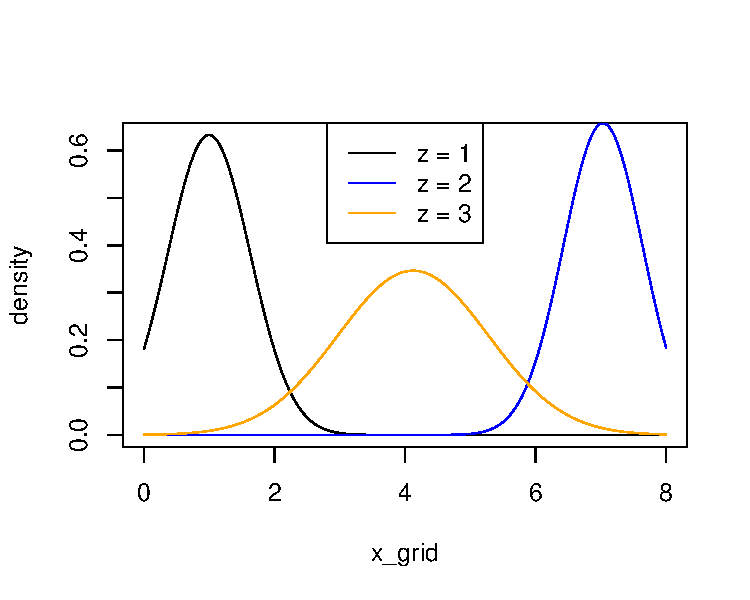
\includegraphics[width=\maxwidth]{figure/unnamed-chunk-11-1} 
\end{knitrout}
    \item[(iii)] Variances would be all equal. Assumption of LDA is equal 
    variances, i.e., estimatated models will always have equal variances, no 
    matter if this fits the data or not
    \item[(iv)] Variances seem not to be equal, this is only captured in QDA
  \end{enumerate}  
  \item Given are two new observations $\xv_{*1} = -10$ and $\xv_{*2} = 7$. 
  State the prediction for each of the two models 
  \begin{enumerate}
    \item[(i)] $\hat{y}_{*1} = 2$, $\hat{y}_{*2} = 3$, 
    \item[(ii)] $\hat{z}_{*1} = 3$, since the variance of class 3 is higher, 
    the density will overshoot the density of class 1. 
    $\hat{z}_{*2} = 2$, obviously highest posterior here.
  \end{enumerate}
  and explain how you derived the predictions.
  \item E.g., 
  \begin{itemize}
    \item CART better than LM because I do not have to specify those indicator 
    functions manually and estimate the split points manually, CART does this 
    data driven
    \item For QDA we have to throw away information of y, this favors CART
    \item QDA predicts the middle class (3) for very extreme observations, this 
    does not seem right. However, we do not know how data behave outside the 
    bounds of x.
    \item QDA assumes gaussian distributions which is clearly not the case.
  \end{itemize}
\end{enumerate}

}

% ------------------------------------------------------------------------------

\newpage
\aufgabeexam{WS2020/21}{main}{3}{

Consider a binary classification algorithm that yielded the following results 
on 8 observations. The table shows  true classes and  predicted probabilities
for class 1:

\begin{tabular}{ | c | c | c | }
  \hline
  ID & True Class & Prediction  \\ \hline
  1 & 1 & 0.50  \\
  2 & 0 & 0.01  \\
  3 & 0 & 0.90  \\
  4 & 0 & 0.55  \\
  5 & 1 & 0.10  \\
  6 & 1 & 0.72  \\
  7 & 1 & 0.70  \\
  8 & 1 & 0.99  \\
  \hline
\end{tabular}

\begin{enumerate}
  \item Draw the ROC curve of the classifier manually. Explain every step 
  thoroughly, and make sure to annotate the axes of your plot.
  \item Calculate the AUC of the classifier. Explain every step of your 
  computation thoroughly.
  \item Calculate the partial AUC for FPR $\leq 1/3$. Explain every step of your 
  computation thoroughly.
  \item Create a confusion matrix assuming a threshold of 0.75. Point out which 
  values correspond to true positives (TP), true negatives (TN), false positives 
  (FP), and false negatives (FN).
  \item Compute sensitivity, specificity, negative predictive value, positive 
  predictive value, accuracy and F1-score. State the respective formulas first.
  \item In the following plot, you see the ROC curves of two different 
  classifiers with similar AUC's. Describe a practical situation where you would 
  prefer classifier 1 over classifier 2 and explain why. (Note: The data in this 
  question is not related to the data of the above questions.)

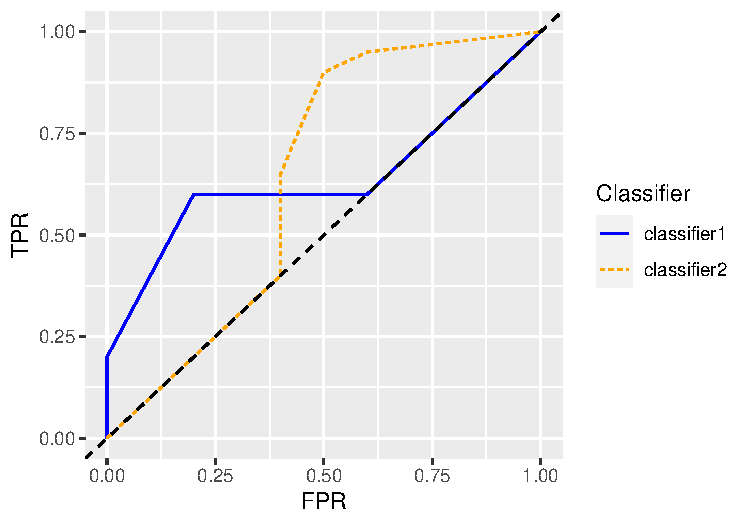
\includegraphics[width=\maxwidth]{figure/unnamed-chunk-12-1} 

\end{enumerate}

}

\dlz
\loesung{

\begin{enumerate}

  \item Scores: \\
\begin{knitrout}
\definecolor{shadecolor}{rgb}{0.969, 0.969, 0.969}\color{fgcolor}
\begin{tabular}{l|r|r}
\hline
  & true\_labels & scores\\
\hline
8 & 1 & 0.99\\
\hline
3 & 0 & 0.90\\
\hline
6 & 1 & 0.72\\
\hline
7 & 1 & 0.70\\
\hline
4 & 0 & 0.55\\
\hline
1 & 1 & 0.50\\
\hline
5 & 1 & 0.10\\
\hline
2 & 0 & 0.01\\
\hline
\end{tabular}

\end{knitrout}
  Here we see that $\frac{1}{n_+} = \frac{1}{5} = 0.2$ and $\frac{1}{n_-} = 
  \frac{1}{3}$. Now we follow the algorithm as described in the lecture slides:
  \begin{itemize}
    \item Set  $\tau = 1$, so we start in $(0,0)$; we predict everything as 1.
    \item Set  $\tau = 0.95$ yields TPR $0 + \frac{1}{n_+} = 0.2$ and FPR  0. 
    (Obs. 8 is '1')
    \item Set  $\tau = 0.8$ yields TPR $0.2$ and FPR  $0 + \frac{1}{n_-} = 1/3$. 
    (Obs. 3 is '0')
    \item Set  $\tau = 0.71$ yields TPR $0.2 + \frac{1}{n_+} = 0.4$ and FPR  
    $1/3$. (Obs. 6 is '1')
    \item Set  $\tau = 0.6$ yields TPR $0.4 + \frac{1}{n_+} = 0.6$ and FPR  
    $1/3$. (Obs. 7 is '1')
    \item Set  $\tau = 0.52$ yields TPR $0.6$ and FPR  $1/3 + \frac{1}{n_-} = 
    2/3$. (Obs. 4 is '0')
    \item Set  $\tau = 0.3$ yields TPR $0.6+ \frac{1}{n_+} = 0.8$ and FPR  
    $2/3$. (Obs. 1 is '1')
    \item Set  $\tau = 0.05$ yields TPR $0.8 + \frac{1}{n_+} = 1$ and FPR  
    $2/3$. (Obs. 5 is '1')
    \item Set  $\tau = 0$ yields TPR $1$ and FPR  $2/3 + \frac{1}{n_-} = 1$. 
    (Obs. 2 is '0')
  \end{itemize}
  Therefore we get the polygonal path consisting of the ordered list of vertices 
  \[(0,0), (0,0.2), (1/3,0.2), (1/3,0.4), (1/3,0.6), (2/3,0.6), (2/3,0.8), 
  (2/3, 1), (1, 1).\]
\begin{knitrout}
\definecolor{shadecolor}{rgb}{0.969, 0.969, 0.969}\color{fgcolor}
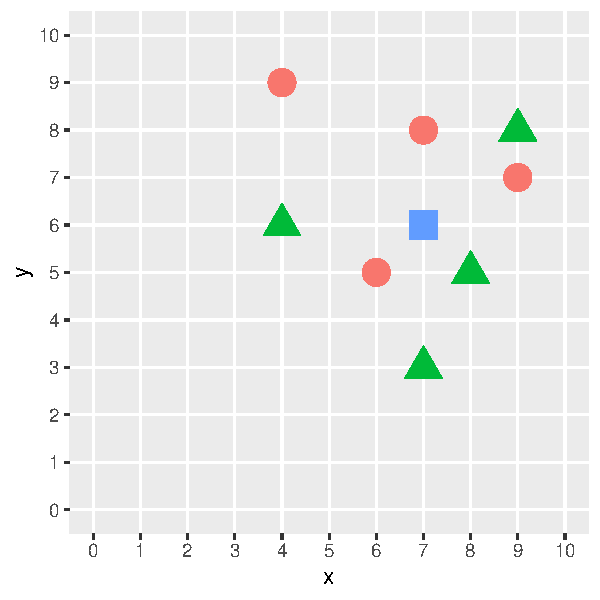
\includegraphics[width=\maxwidth]{figure/unnamed-chunk-14-1} 
\end{knitrout}
  
  \item The AUC is the sum of three rectangles: $0.2 \cdot 1/3 + 0.6 \cdot 1/3 + 
  1\cdot 1/3 = 0.6$
  
  \item The partial AUC is the area under the curve that is left from 
  FPR $= 1/3$, so it is just the first rectangle: $0.2 \cdot 1/3 = 1/15$
  
  \item \phantom{foo}
  \begin{tabular}{ | c | c | c | } \hline
    & Actual Class - 0 & Actual Class - 1  \\
    Prediction - 0 & 2 & 4  \\
    Prediction - 1 & 1 & 1  \\ \hline
  \end{tabular}
  so we get
  \begin{tabular}{ | c | c | c | c | }
    \hline
    FN & FP & TN & TP   \\ \hline
    4 & 1 & 2 & 1 \\ \hline
  \end{tabular}
    
  \item $$\text{Sensitivity} = \frac{\text{TP}}{\text{TP} + \text{FN}} =
  \frac{1}{5} $$
  $$\text{Specificity}  = \frac{\text{TN}}{\text{TN} + \text{FP}} =\frac{2}{3}$$
  $$\text{Negative Predictive Value} = \frac{\text{TN}}{\text{TN} + \text{FN}} =
  \frac{1}{3} $$
  $$\text{Positive Predictive Value} = \frac{\text{TP}}{\text{TP} + \text{FP}} =
  \frac{1}{2} $$
  $$\text{Accuracy} = \frac{\text{TP} + \text{TN}}{\text{TP} + \text{TN} + 
  \text{FP} + \text{FN}} =\frac{3}{8} $$
  $$\text{F1-score} = \frac{2\cdot\text{PPV}\cdot\text{Sensitivity}}{\text{PPV}
  +\text{Sensitivity}} = (0.2) / (0.7) = 2/7  $$
  
  \item Important point is to understand that classifier 1 does better in the
  'high scores'. Or: For some threshold below 0.5 the precision is far better
  for classifier 1 than for classifier 2. For example if you want to output a
  certain number of 'most promising customers' this could be a good idea.

\end{enumerate}
}

% ------------------------------------------------------------------------------

\dlz
\aufgabeexam{WS2020/21}{main}{4}{

The table below shows $\D = \Dset $, a data set with 
$n$ = 8 observations of a binary target variable $y$ containing the information 
if the object is a \texttt{Banana} or not and a 4-dimensional feature vector 
$\xv$, containing \texttt{Color}, \texttt{Form}, \texttt{Origin} (categorical 
features) and \texttt{Length} (continuous feature) of the object. In the 
following, we aim at predicting \texttt{Banana} with a machine learning model 
that takes $\xv$ as input.

\begin{tabular}{ | c | c | c | c | c | c |}
\hline
ID  &  Color   &  Form    &  Origin    & Length [cm]  &  Banana  \\  \hline
1   &  yellow  &  oblong  &  imported  & 15           &  yes      \\
2   &  yellow  &  round   &  domestic  & 5            &  no       \\
3   &  yellow  &  oblong  &  imported  & 10           &  no       \\
4   &  brown   &  oblong  &  imported  & 17           &  yes      \\
5   &  brown   &  round   &  domestic  & 16           &  no        \\
6   &  green   &  round   &  imported  & 13           &  yes       \\
7   &  green   &  oblong  &  domestic  & 25           &  no       \\
8   &  red     &  round   &  imported  & 7            &  no        \\
\hline
\end{tabular}

We want to use a naive Bayes classifier to predict the label of a new 
observation. 

\begin{enumerate}
  \item Calculate the posterior probability $\pi(\xv_*) = \P(y = \text{yes} | 
  \xv_*)$ for a new observation \ $\xv_* = (\text{green}, \text{oblong}, 
  \text{imported}, 14)^\top$. Explain every step thoroughly. (Hint: At some 
  point you will have to compute values of Gaussian densities - use R for this
  step.)
\end{enumerate}

}

\dlz
\loesung{

\begin{enumerate}

  \item The features $\xv := (x_\text{Color},x_\text{Form},x_\text{Origin},
  x_\text{Length})$ given the category $y \in \{\text{yes},\text{no}\}$ are
  assumed to be conditionally independent of each other (since we are using
  Naive Bayes), s.t.

  $$p(\xv|y = k) = p(x_\text{Color}|y = k)\cdot p(x_\text{Form}|y = k) \cdot
  p(x_\text{Origin}|y = k) \cdot p(x_\text{Length}|y = k).$$

  For the posterior probabilities $\pi_k(\xv) = \P(y = k | \xv)$ it holds with
  Bayes' Theorem:
  \begin{align*}
  \pi_k(\xv)  \propto & \; \underbrace{\pi_k \cdot p(\xv|y = k)
  }_{=: \alpha_k(\xv)} \\
  \iff & \exists c \in \mathbb{R}: \pi_k(\xv) = c \cdot \alpha_k(\xv),
  \end{align*}

  where $\pi_k = \P(y = k)$ is the prior probability of class $k$.

  From this and since the posterior probabilities need to sum up to 1, it holds
  that
  \begin{align*}1 =& \; c \cdot \alpha_\text{yes}(\xv) +  c \cdot
  \alpha_\text{no}(\xv) \\
  \iff & c = \frac{1}{\alpha_\text{yes}(\xv) + \alpha_\text{no}(\xv)}.
  \end{align*}

  This means, the scores $\alpha_\text{yes}(x)$ and $\alpha_\text{no}(x)$ are
  needed to compute  $$\pi_\text{yes}(\xv) = \frac{\alpha_\text{yes}(\xv)}{
  \alpha_\text{yes}(\xv) + \alpha_\text{no}(\xv)}. $$

  For the new observation $\xv_*$ we have to estimate the respective
  probabilities and densities. For the categorical features, we can simply
  compute relative frequencies. For the continuous features \texttt{Length} we
  have to estimate the densities per class and evaluate those at the value $14$.
  Doing this with R we end up with:

\begin{knitrout}
\definecolor{shadecolor}{rgb}{0.969, 0.969, 0.969}\color{fgcolor}\begin{kframe}
\begin{verbatim}
## [1] 0.1760327
## [1] 0.04863352
\end{verbatim}
\end{kframe}
\end{knitrout}

  \begin{center}
  \begin{tabular}{ | c | c | c | c | c | c |}
  \hline
  k     &  $\hat{\pi}_k$   &  $\hat{p}(\text{green}|y = k)$    &  
  $\hat{p}(\text{oblong}|y = k)$    & $\hat{p}(\text{imported}|y = k)$    & 
  $\hat{p}(\text{14}|y = k)$   \\  \hline
  yes   &  3/8  &  1/3    &  2/3  & 3/3     &  0.176 \\
  no    &  5/8  &  1/5    &  2/5  & 2/5     &  0.049 \\
  \hline
  \end{tabular}
  \end{center}

  \begin{align*}
  \hat{\alpha}_\text{yes}(x) = & \;  \hat{\pi}_{yes} \cdot \hat{p}(
  \text{green}|y = \text{yes})\cdot \hat{p}(\text{oblong}|y = \text{yes}) \cdot 
  \hat{p}(\text{imported}|y = \text{yes}) \cdot \hat{p}(14|y = \text{yes}) \\
  = & \; \frac{3}{8} \cdot \frac{1}{3} \cdot \frac{2}{3} \cdot 1 \cdot 0.176  
  \approx 0.0147, \\
  \hat{\alpha}_\text{no}(x) = & \;  
  \hat{\pi}_{no} \cdot \hat{p}(\text{green}|y = \text{no})\cdot 
  \hat{p}(\text{oblong}|y = \text{no}) \cdot \hat{p}(\text{imported}|y = 
  \text{no}) \cdot \hat{p}(14|y = \text{no}) \\
  = & \; \frac{5}{8} \cdot \frac{1}{5} \cdot \frac{2}{5} \cdot \frac{2}{5} 
  \cdot 0.049  \approx 0.00098.
  \end{align*}
  
  With this we can calculate the posterior probability
  $$\hat{\pi}_\text{yes}(x) = \frac{\hat{\alpha}_\text{yes}(x)}{\hat{\alpha}_\text{yes}(x) + \hat{\alpha}_\text{no}(x)} \approx 0.937.$$

\end{enumerate}
}

% ------------------------------------------------------------------------------
% INSPO
% ------------------------------------------------------------------------------

\dlz
\exinspo
\end{document}
